
\section{Propriétés}
\label{net:sec:properties}

\SPRAY est un protocole d'échantillonnage aléatoire de pair adaptatif. Cette
section a pour objectif d'examiner ses propriétés empiriquement au travers une
série de simulations. Les métriques auxquelles nous nous intéressons sont
communément employées dans l'étude de performances de ce type de protocoles ou
en étude des graphes. Ceux-ci incluent le coefficient d'agglomération
(\emph{clustering coefficient}), la taille moyenne du plus court chemin, la
distribution des connexions entrantes, l'évolution du nombre d'arcs, les
composantes connexes, et la robustesse. À cela nous ajoutons une analyse sur les
doublons d'arcs, spécificité de \SPRAY.

% \TODO{Review this §.}
% \CYCLON constitue l'approche à taille fixe avec laquelle nous comparerons les
% résultats en lien avec l'adaptabilité. Les résultats attendus sont :
% \begin{inparaenum}
% \item des propriétés identiques pour les deux approches lorsque \CYCLON est
%   configuré de manière optimale,
% \item une meilleure efficacité de \SPRAY lorsque les vues partielles de \CYCLON
%   sont trop grande par rapport à la taille du réseau,
% \item une plus grande robustesse lorsque les vues partielles de \CYCLON sont
%   trop petites par rapport à la taille du réseau.
% \item Enfin, contrairement à \CYCLON, \SPRAY possède des doublons dans ses vues
%   partielles. Toutefois, ce nombre de doublons est supposé négligeable.
% \end{inparaenum}
% \SCAMP constitue l'approche avec laquelle nous comparerons \SPRAY lorsque nous
% examinerons les échecs dans l'établissement des connexions. Nous nous attendons
% à ce que \SCAMP échoue à maintenir un réseau connecté, contrairement à \SPRAY.

Les expérimentations ont été effectuées sur le simulateur
\PEERSIM~\cite{montresor2009peersim}. Le code relatif aux protocoles
d'échantillonnages \CYCLON, \SCAMP, et \SPRAY sont disponibles sur la
plate-forme Github à l'adresse : \url{http://github.com/justayak/peersim-spray}.

\subsection{Coefficient d'agglomération}
\label{net:subsec:clustering}

\begin{figure*}
  \centering
  \subfloat[Coefficient d'agglomération de \CYCLON.]
  [Coefficient d'agglomération de \CYCLON.]
  {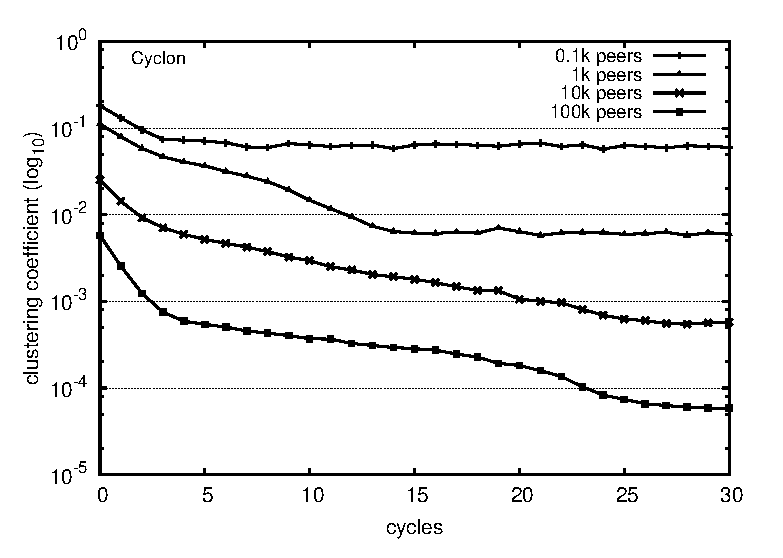
\includegraphics[width=0.47\textwidth]{img/spray/cycloncluster.eps}}
  \hspace{10pt}
  \subfloat[Coefficient d'agglomération de \SPRAY.]
  [Coefficient d'agglomération de \SPRAY.]
  {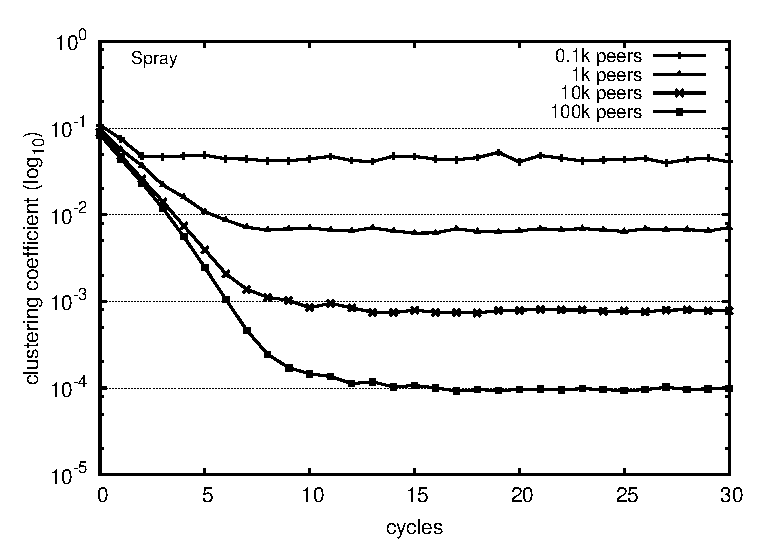
\includegraphics[width=0.47\textwidth]{img/spray/spraycluster.eps}}
  \caption{\label{net:fig:clustering}L'axe des abscisses marque le temps écoulé
    en nombre de cycles. L'axe des ordonnées note le coefficient d'agglomération
    sur une échelle logarithmique de base 10.}
\end{figure*}

Le coefficient d'agglomération désigne une mesure de groupement des nœuds. En
d'autres termes, si un petit groupe possède un grand nombre d'arcs les reliants,
alors la mesure grimpe. Ainsi, les graphes complets affichent un coefficient
maximal. À l'inverse, les graphes aléatoires affichent un coefficient très bas
car la répartition des arcs ainsi que leur nombre ne favorise pas l'apparition
de groupes.

Si le comportement de cette métrique fait consensus, il existe malgré tout
plusieurs formules pour la calculer. Dans cette simulation, nous employons le
coefficient local moyen $\overline{C}$~\cite{watts1998collective} effectuant la
moyenne du coefficient $C_x$ de chaque nœud $n_x$ :
\begin{center}
  $\overline{C} = {1\over |\mathcal{N}|}\sum\limits_{x\in\mathcal{N}}C_x$ \hfill
  avec
  $C_x = {|\{ (n_y,\,n_z) \in P_x, n_y \in P_z \vee n_z \in P_y \}|\over
    |P_x|.(|P_x|-1)}$
\end{center}

\begin{itemize}
\item [\textbf{Objectif :}] Montrer que \SPRAY converge rapidement vers une
  topologie ne comportant pas de groupes fortement connexes.
\item [\textbf{Description :}] Les simulations ciblent des réseaux composés
  respectivement de 0.1k, 1k, 10k, et 100k nœuds. Le représentant des approches
  à taille fixe est \CYCLON. Ce dernier est configuré de manière optimale pour
  1k pairs ($\ln(1000)\approx 7$ voisins). De plus, les nœuds utilisant \CYCLON
  échangent 3 de leurs 7 voisins à chaque mélange.
\item [\textbf{Résultat :}] La figure~\ref{net:fig:clustering} montre que
  \CYCLON démarre avec un coefficient d'agglomération plus bas que
  \SPRAY. Malgré cela, \SPRAY parvient à converger plus rapidement que
  \CYCLON. De plus, quand le nombre de nœuds augmente dans le réseau, le temps
  de convergence de \CYCLON en souffre fortement. À l'opposé, \SPRAY converge
  très rapidement quel que soit la taille du réseau. La
  figure~\ref{net:fig:clustering} montre aussi que les deux approches convergent
  vers un petit coefficient caractéristique des graphes aléatoires. Néanmoins,
  \CYCLON et \SPRAY n'atteignent pas les mêmes valeurs après convergence. À
  l'exception du cas où \CYCLON est configuré de manière optimale, les valeurs
  obtenues par \SPRAY sont soit au dessous -- lorsque les vues de \CYCLON sont
  trop grandes -- ou au dessus -- lorsque les vues de \CYCLON sont trop
  petites. Globalement, \SPRAY
  \begin{inparaenum}[(i)]
  \item converge vers un coefficient d'agglomération stable
  \item reflètant les besoins dûs à la taille du réseau.
  \end{inparaenum}
%%  Cela a une influence sur l'équilibrage des charges et la robustesse par
%%  rapport aux allées et venues de pairs.    
\item [\textbf{Explication :}] \CYCLON commence avec un coefficient
  d'agglomération plus faible car lorsqu'un nœud rejoint le réseau, il est
  annoncé au reste du réseau via une dissémination aléatoire. Ainsi, le réseau
  de départ est déjà légèrement équilibré au moment où la simulation commence. À
  l'opposé, un nouvel arrivant \SPRAY n'annonce son entrée qu'au voisinage de
  son contact. De ce fait, le réseau est fortement déséquilibré au départ de
  l'expérience quelle que soit taille du réseau. Malgré cela, \CYCLON ne
  converge pas aussi vite que \SPRAY vers un coefficient stable. En effet, la
  taille fixe de sa vue partielle ainsi que le nombre d'entrées de chaque
  mélange contraint la qualité des échanges.  Le coefficient d'agglomération
  mesure la connexité du voisinage de chaque nœud. Plus particulièrement, cela
  mesure à quel point le réseau est proche d'un graphe complet. Cela dépend donc
  des tailles de vue partielle qui, pour \CYCLON, sont fixées à la
  configuration.  Ainsi lorsque le nombre de nœuds est multiplié par 10, le
  coefficient s'en trouve divisé par 10. En revanche, les nœuds utilisant \SPRAY
  ont une taille de vue partielle reflétant automatiquement la taille du réseau.
  Ainsi, quand le réseau contient 1k nœuds, les vues partielles s'adaptent à
  cette taille. Par conséquent, \SPRAY est très légèrement en dessous de \CYCLON
  dans ce scénario car la taille moyenne de vue partielle est de 7.4 pour ce
  premier contre 7 pour ce second. En étendant ce raisonnement aux autres
  tailles de réseau, cela explique pourquoi \SPRAY converge vers une valeur plus
  basse lorsque les vues partielles de \CYCLON sont trop grandes (0.1k nœuds),
  et vers une valeur plus haute lorsque les vues partielles de \CYCLON sont trop
  petites (10k et 100k nœuds).
\end{itemize}

\subsection{Plus court chemin moyen}
\label{net:subsec:shortestpath}

\begin{figure}
  \centering
  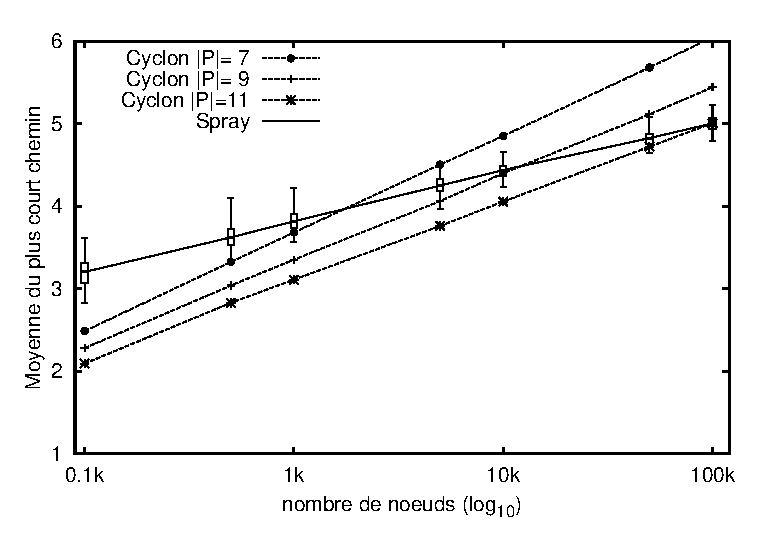
\includegraphics[width=.8\textwidth]{img/spray/avgpath.eps}
  \caption{\label{net:fig:shortestpath} La moyenne des plus courts chemins dans
    \SPRAY et \CYCLON. L'axe des abscisses montre le nombre de nœuds appartenant
    aux réseaux sur une échelle logarithmique de base 10. L'axe des ordonnées
    montre la moyenne des plus courts chemins.}
\end{figure}

La moyenne des plus courts chemins permet de mesurer à quel point les nœuds sont
proches les un des autres. Plus précisément, il s'agit de compter le nombre
minimum de nœuds intermédiaires entre deux nœuds distincts. Ainsi, même s'il
existe plusieurs chemins pour aller d'un nœud $n_i$ à un nœud $n_j$, seul nous
importe le plus court.  Les graphes aléatoires possèdent un plus court chemin
moyen très petit grandissant en $\ln|\mathcal{N}|\over\ln\ln|\mathcal{N}|$
lorsque le nombre d'arcs suit $|\mathcal{N}|\ln|\mathcal{N}|$.

Cette métrique permet de cerner l'efficacité de la diffusion d'informations dans
le réseau. Par exemple, si le plus court chemin d'un nœud $n_i$ à un nœud $n_j$
est de 3, cela signifie qu'un message émanant de $n_i$ parviendra en seulement 3
intermédiaires à $n_j$.

\begin{itemize}
\item [\textbf{Objectif :}] Montrer que le caractère adaptatif de \SPRAY permet
  un meilleur passage à l'échelle du plus court chemin moyen.
\item [\textbf{Description :}] Les mesures sont effectuées sur un sous-ensemble
  de nœuds choisis aléatoirement parmis les membres du réseau. Le procédé est
  répété 100 fois afin d'éviter tout effets de bord dû à l'indéterminisme des
  protocoles d'échantillonnage. Les expérimentations concernent \CYCLON
  configuré de façon optimale pour différentes tailles de réseau. Le \CYCLON
  avec une taille de vue partielle de 7 cible environ 1.1k nœuds. Le \CYCLON
  avec une taille de vue partielle de 9 cible environ 8.1k nœuds. Le \CYCLON
  avec une taille de vue partielle de 11 cible environ 60k nœuds. Lors de toutes
  ces simulations, les mesures sont effectuées après convergence. Celles-ci sont
  faites lorsque la taille du réseau atteint 0.1k, 0.5k, 1k, 5k, 10k, 50k, et
  100k nœuds.
\item [\textbf{Résultat :}] La figure~\ref{net:fig:shortestpath} montre que
  \CYCLON et \SPRAY ont tous deux un chemin moyen relativement petit. Ainsi, les
  informations peuvent être disséminées à tous les membres du réseau très
  rapidement. La figure~\ref{net:fig:shortestpath} montre aussi que chaque
  exécution de \CYCLON prise séparément peut être divisée en trois phases.  Tout
  d'abord, la phase où les vues partielles de \CYCLON sont trop grandes
  dissémine l'information plus rapidement que \SPRAY. Lors les vues partielles
  sont optimales, \CYCLON et \SPRAY montrent des résultats similaires. Enfin,
  \SPRAY montre une meilleure efficacité lorsque les vues partielles de \CYCLON
  sont trop petites. Malgré tout, \SPRAY passe mieux à l'échelle que \CYCLON
  l'inclinaison de cette première est inférieure à n'importe quelle
  configuration de cette dernière.
\item [\textbf{Explication :}] Les mesures sont toutes effectuées après
  convergence, lorsque les réseaux possèdent une topologie proche des graphes
  aléatoires.  Dans de tels graphes, la taille du plus court chemin moyen reste
  petit.  La seconde observation concerne chacune des configurations de \CYCLON
  comparée à \SPRAY. Une taille de vue partielle surestimée pour \CYCLON est
  meilleure en terme de connexité entre nœuds et résulte dans de plus courts
  chemins en moyenne. En revanche, dès que cette taille devient insuffisante
  pour le réseau, \SPRAY devient plus efficace car il possède de plus grandes
  vues partielles. Puisque \SPRAY suit toujours la taille optimale de vue
  partielle, il passe mieux à l'échelle en terme de taille réseau.
\end{itemize}

\subsection{Distribution des arcs entrants}
\label{net:subsec:inview}

\begin{figure}
  \centering
  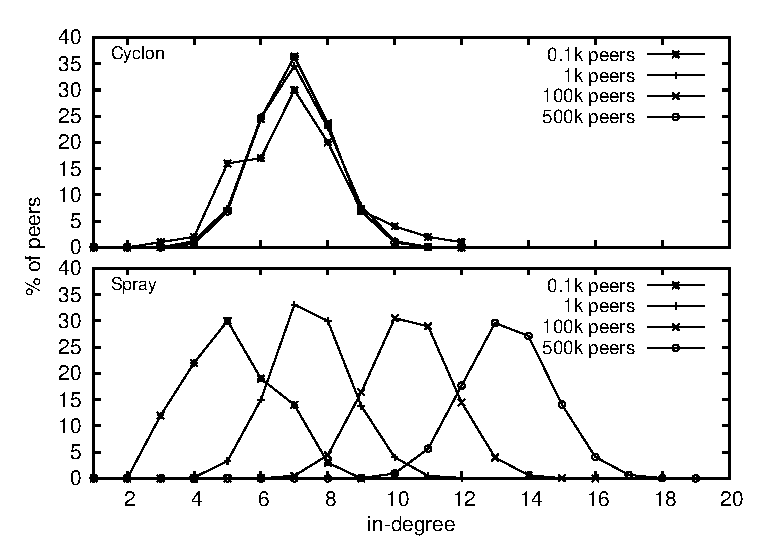
\includegraphics[width=.8\textwidth]{img/spray/histo.eps}
  \caption{\label{net:fig:inview} Distribution du nombre d'arcs entrants à
    chaque nœud dans \CYCLON et \SPRAY. L'axe des ordonnées montre la proportion
    de nœuds ayant une vue entrante de la taille correspondante sur l'axe des
    abscisses. Les figure du haut et du bas sont respectivement dédiées aux
    exécutions concernant \CYCLON et \SPRAY.}
\end{figure}

La distribution des arcs entrants correspond au nombre de fois qu'un nœud est
référencé dans une vue partielle. À cet égard, la distribution est différentes :
Lorsque la taille des vues partielles est controllée, les vues entrantes sont
aléatoirement remplies par d'autres nœuds au cours de l'exécution du
protocole. Certains nœuds sont donc moins représentés que d'autres.  Au même
titre que la distribution des vues partielles, la distribution des arcs sortants
permet de déduire des faits sur la robustesse du réseau, l'équilibre de la
charge etc. 

\begin{itemize}
\item [\textbf{Objectif :}] Montrer que la distribution des arcs entrants dans
  \SPRAY suit gracieusement l'évolution du réseau.
\item [\textbf{Description :}] Dans cette expérimentation, \CYCLON est configuré
  avec une vue partielle contenant 7 voisins (optimal pour 1.1k nœuds). Les
  mesures sont effectuées après convergence sur des réseaux comprenant : 0.1k,
  1k, 100k, 500k nœuds.
\item [\textbf{Résultat :}] Le haut et le bas de la figure~\ref{net:fig:inview}
  montrent la distribution des connexions entrantes pour \CYCLON et \SPRAY,
  respectivement. Nous observons que \CYCLON possède une distribution identique
  quelle que soit la taille du réseau. La distribution d'un réseau de 0.1k nœuds
  est identique à celle de 500k nœuds, avec un fort pic sur la valeur moyenne de
  7 voisins. À l'opposé, la distribution des connexions entrantes de \SPRAY suit
  la taille du réseau. La figure~\ref{net:fig:inview} montre que les nœuds sont
  très concentrés autour des valeurs moyennes. Par exemple, lors de l'exécution
  du protocole \SPRAY avec 500k nœuds, la moyenne est de 13.37 avec 88\% des
  nœuds compris entre 12 et 14 voisins inclus. Entre autre, cela signifie que la
  charge est très équilibrée parmi les nœuds. Puisque chaque nœud est aussi
  important que son voisin en terme de connexité, le réseau est robuste
  vis-à-vis des défaillances.
\item [\textbf{Explication :}] Une fois configuré, \CYCLON doit gérer tous les
  réseaux, quelle que soit leur taille, avec une vue partielle dont la taille
  est constante. Proportionnellement, le nombre de fois qu'un nœuds est
  référencé dans les vues partielles ne change pas comparé à la taille
  réseau. En effet, le nombre d'arcs qu'un nœud apporte lorsqu'il se connecte au
  réseau constitue autant d'arcs le ciblant après quelques protocoles
  d'échanges. Puisque la taille de la vue partielle est constante, le degré des
  connexions entrantes reste stable. En revanche, dans \SPRAY, chaque nœuds
  rejoignant le réseau augmente le nombre d'arcs dans le réseau. Ainsi, le degré
  de connexions entrantes de chaque nœud grossit reflétant les variations du
  réseau. Par conséquent, la distribution de \SPRAY se décale lentement vers de
  plus hautes valeurs lorsque la taille du réseau augmente. \SPRAY ne possède
  pas de pics sur les valeurs moyennes car celles-ci sont des valeurs qui
  tombent entre deux entiers. Par exemple, si la taille moyenne des vues
  partielles est 6.5, cela signifie que la moitié de celle-ci ont une taille de
  6, et l'autre moitié une taille de 7. De tels réseaux sont robustes aux
  défaillances car aucun nœud n'est plus important que son voisin en terme de
  connexité. Si un nœud particulier quitte ou défaillit, les nœuds le
  référençant possèdent d'autres voisins avec qui communiquer afin de continuer
  à disséminer les informations.
\end{itemize}

\subsection{Évolution du nombre d'arcs}
\label{net:subsec:churn}

\begin{figure*}
  \centering 
  \subfloat[Nombre d'arcs et variance du réseau.]
  [\label{net:fig:churnA} L'axe des abscisses montre le temps écoulé en terme de
  cycles. L'axe des ordonnées de la figure du haut montre le nombre total d'arcs
  dans le réseau tandis que l'axe des ordonnées de la figure du bas montre la
  variance $\sigma^2$ de la taille des vues partielles.]
  {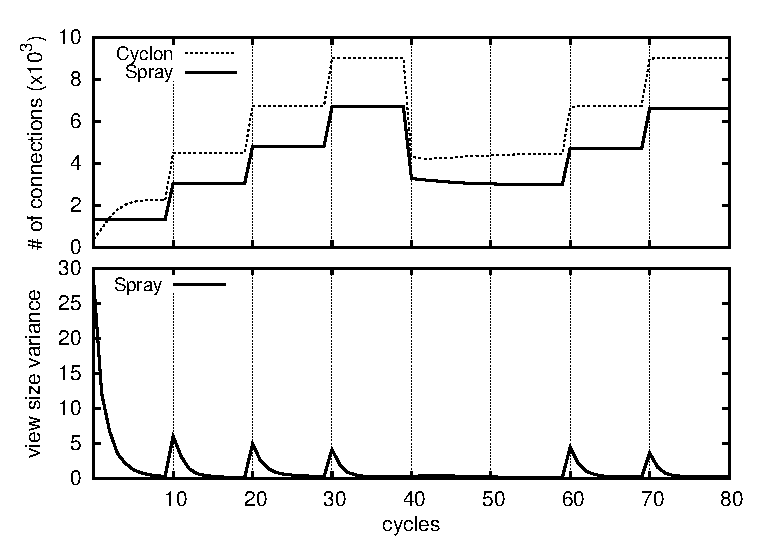
\includegraphics[width=0.47\textwidth]{img/spray/churn.eps}}
  \hspace{10pt}
  \subfloat[Taille moyenne des vues partielles.]
  [\label{net:fig:churnB} L'axe des abscisses montre le temps écoulé en terme de
  cycles. L'axe des ordonnées montre la taille moyenne des vues partielles.]
  {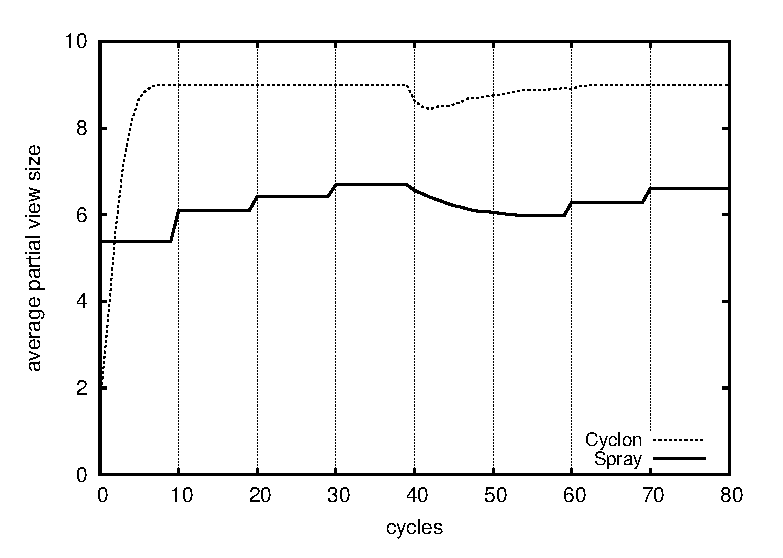
\includegraphics[width=0.47\textwidth]{img/spray/avgpv.eps}}
  \caption{\label{net:fig:churn} Évolution du nombre d'arcs dans un réseau
    dynamique : 250 nœuds rejoignent le réseau aux cycles $0$, $10$, $20$, et
    $30$. Puis 500 nœuds quittent le réseau au cycle $40$. Enfin, 250 nœuds
    rejoignent le réseau au cycles $60$ and $70$. Au plus haut, le réseau
    comprend 1k nœuds.}
\end{figure*}

Un réseau est dynamique lorsque des nœuds peuvent le rejoindre et le quitter --
ce qui compose la plupart des cas en pratique. Le protocole d'échantillonnage
doit être capable de gérer efficacement de tels changements. La variance d'un
ensemble de valeurs permet de quantifier les différences qu'il existe entre les
valeurs. Appliquée aux tailles de vues partielles, cette mesure permet
d'observer l'évolution du système supposé convergeant. Une variance de 0
signifie que toutes les valeurs de l'ensemble sont identiques.

\begin{itemize}
\item [\textbf{Objectif :}] Montrer l'évolution logarithmique du nombre d'arcs
  des vues partielles dans un réseau dont les nœuds entrent et sortent du réseau
  au cours du temps. Montrer qu'à chaque changement du réseau, le système
  converge en temps exponentiel vers des vues partielles dont la taille est
  proche.
\item [\textbf{Description :}] La configuration de \CYCLON cible un réseau de
  taille 8.1k nœuds, soit des vues partielles configurées à 9 voisins. Sachant
  qu'au plus haut la simulation comprend 1k nœuds, cela signifie que la vue
  partielle a été volontairement surestimée. Lors de la première moitié de la
  simulation, 4 groupes successifs comportant 250 nœuds rejoignent le
  réseau. L'intervalle de temps entre ces entrées est de 10 cycles. Ainsi, le
  réseau initialement vide contient 1k nœuds au bout de 40 cycles. Ensuite, la
  moitié des membres du réseau le quitte, soit un départ de 500 nœuds d'un
  coup. Enfin, 2 groupes de 250 nœuds rejoignent le réseau à nouveau faisant
  passer la taille de celui-ci à 1k nœuds. Les mesures concernent
  \begin{inparaenum}[(i)]
  \item le nombre de connexions dans le réseau au cours du temps,
  \item la variance de la taille des vues partielles au cours du temps,
  \item la taille moyenne des vues partielles au cours du temps.
  \end{inparaenum}
\item [\textbf{Résultat :}] La figure~\ref{net:fig:churn} montre les résultats
  de cette expérimentation. La partie haute de la figure~\ref{net:fig:churnA}
  montre le nombre d'arcs créés dans le réseau sur une échelle $\times 10^3$)
  tandis que la partie basse de la figure montre la variance de taille des vues
  partielles de \SPRAY. Dans le cas des deux protocoles d'échantillonnage, nous
  observons qu'à chaque groupe rejoignant le réseau, le nombre de connexions
  augmente. Toutefois, la suréstimation de \CYCLON place son nombre d'arcs au
  dessus de \SPRAY (entre 1k et 2.5k arcs supplémentaire). De plus, la
  figure~\ref{net:fig:churnB} montre que les vues partielles de \CYCLON restent
  de taille constante pendant toute la simulation excepté lors des départs du
  $40$\up{ème} cycle où les vues sont petit à petit purgées des arcs
  obsolètes. \SPRAY hérite de ce dernier trait. En revanche, les vues partielles
  s'adaptent automatiquement aux changements du réseau. Cette progression est
  logarithmique et lorsque le réseau comprend 1k nœuds, les vues partielles de
  \SPRAY ont pour taille moyenne 6.6 voisins ($\ln(1000)\approx6.9$). La partie
  basse de la figure~\ref{net:fig:churnB} montre que les vues partielles
  s'équilibrent extrêmement rapidement. Notamment les premiers cycles qui
  réduisent considérablement l'écart entre vues partielles. La figure montre
  aussi que les départs ne déséquilibrent pas les vues partielles.
\item [\textbf{Explication :}] Puisque les vues partielles de \SPRAY s'adaptent
  à la taille du réseau, le nombre de connexions augmente lorsque des membres
  s'ajoute au réseau. Les pics de variance correspondent à la partie du
  protocole où les nœuds rejoignent le réseau. Les différences en hauteur des
  pics proviennent du fait que les nouveaux arrivant commencent avec une petite
  vue partielle. Les nœuds étant présent avant que le nouveau groupe rejoigne le
  réseau ont eu quelques cycles d'échanges afin d'équilibrer leur vues. Par
  conséquent, le poids des nouveaux arrivant est proportionnellement plus
  faible. Le départ des 500 nœuds au cycle 40 ne perturbe pas la variance car
  ils sont choisis aléatoirement. Ainsi, aucun nœud ne souffre particulièrement
  des départs comparé aux autres nœuds. Toutefois, nous observons une très
  faible décroissance du nombre d'arcs suite à cela. En effet, \CYCLON et \SPRAY
  utilisent tout deux un âge relatif à l'insertion d'un arc dans sa vue
  partielle. À chaque processus périodique de mélange, le plus vieux arc est
  examiné. S'il est obsolète, l'arc est retiré. Par conséquent, ce mécanisme de
  détection prend plusieurs cycles à détecter les départs et défaillances. Plus
  la vue partielle est petite, plus le processus est rapide ce qui fait de
  \SPRAY un processus plus réactif vis-à-vis des départs.
\end{itemize}

\subsection{Robustesse}
\label{net:subsec:robustness}

\begin{figure}
  \centering
  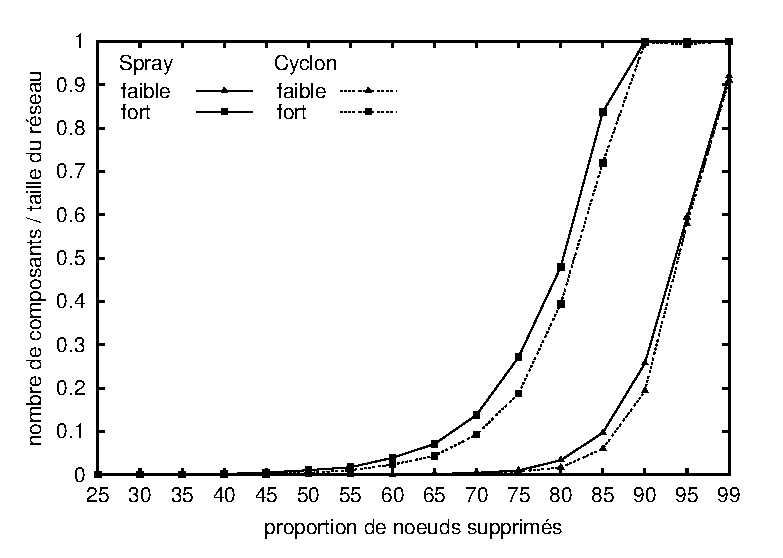
\includegraphics[width=.8\textwidth]{img/spray/resilience.eps}
  \caption{\label{net:fig:robustness} Robustesse de \CYCLON et \SPRAY face aux
    défaillances aléatoires massives. L'axe des abscisses montre le pourcentage
    de nœuds supprimé en une fois. L'axe des ordonnées montre le ratio entre le
    nombre de composantes connexes et la taille du réseau après suppression.}
\end{figure}

La robustesse d'un réseau est sa capacité à rester connexe lorsque des
défaillances apparaissent. Ici, nous ne prenons en compte que les défaillances
aléatoires non-corrélés. Lorsqu'un nœud quitte le réseau, qu'il soit défaillant
ou non, un certain nombre d'arcs deviennent obsolètes. Si ces arcs constituaient
les seuls liens entre deux parties du réseau, alors apparaissent des partitions.
Dans les graphes aléatoires, un grand nombre de nœuds doivent disparaître avant
que de telles partitions apparaissent.

Compter le nombre de composantes fortement connexes dans un réseau permet
d'estimer la surface atteignable par les protocoles de dissémination
d'informations. Par exemple, il y a deux composantes fortement connexes dans un
réseau dont une partie peut atteindre l'autre sans que l'inverse soit
vrai.

Compter le nombre de composantes faiblement connexes dans une réseau permet
d'estimer le moment où celui-ci n'est plus réparable. Un réseau est réparables
si après quelques échanges de vues partielles, les informations peuvent être
disséminées à tous les participants encore dans le réseau. Il suffit d'un lien
entre deux composantes fortement connexes pour que le réseau soit
réparable. Sans ce lien, les composantes sont faiblement connexes.

\begin{itemize}
\item [\textbf{Objectif :}] Montrer que \SPRAY est robuste face aux défaillances
  aléatoires massives.
\item [\textbf{Description :}] \CYCLON est configuré de façon à fournir des vues
  partielles contenant 9 voisins. Le réseau compte 10k membres. Les suppressions
  sont effectuées après convergence. Les nœuds sont supprimés aléatoirement et
  d'un trait. Allant de 25\% à 95\% par paliers de 5\% cela représente 16
  exécutions par approche. La dernière mesure est effectuée à 99\% de
  suppressions. Les mesures des composantes connexes sont effectuées
  immédiatement après suppression.
\item [\textbf{Résultat :}] La figure~\ref{net:fig:robustness} montre le ratio
  de composantes fortement et faiblement connexes du réseau après suppression
  massive de nœuds. Tout d'abord, la figure montre que les deux protocoles
  d'échantillonnage de pairs, \SPRAY et \CYCLON, ne souffrent de partionnement
  qu'après un fort taux de suppressions, \CYCLON étant légèrement meilleur dans
  ce cas. La figure~\ref{net:fig:robustness} montre que les composantes
  fortement connexes commencent à se dégrader lentement dès 45\%, et plus
  rapidement à 70\%. Dans ce cas, la dissémination d'informations est
  temporairement en danger. Heureusement, la figure~\ref{net:fig:robustness}
  montre aussi que ces approches sont capables de réparer ce partionnement. En
  effet, les composantes faiblement connexes ne commencent à augmenter qu'à
  partir de 70\%, ce qui signifie que des parties du réseau sont complètement
  disjointes et donc, au delà de toute possibilité de réparation.
\item [\textbf{Explication :}] Les protocoles d'échantillonnage de pairs \CYCLON
  et \SPRAY affichent des résultats très similaires car \CYCLON est configuré
  pour une taille de réseau de 10k nœuds, tandis que \SPRAY s'ajuste
  automatiquement à cette taille de réseau. Par conséquent, leur nombre d'arcs
  est très proche. Ici, \CYCLON possède légèrement plus de connexions -- car
  \SPRAY possède une part d'aléatoire -- et aucun doublon dans les vues
  partielles -- \SPRAY possède un faible taux de doublons (cf. la
  figure~\ref{net:fig:duplicates}). Afin de mettre en dangers la dissémination
  d'informations, il est nécessaire de supprimer un fort taux de nœuds. En
  effet, chaque nœud revêt grossièrement la même importance que son
  voisin. Ainsi, supprimer des nœuds aléatoirement parmi ceux-ci n'affectent pas
  énormément le réseau dans son entièreté. Le réseau est capable de se réparer
  car les protocoles d'échantillonnage ne dépendent que d'arcs unidirectionnels
  pour fonctionner. Ainsi, s'il subsiste un lien entre deux composantes
  fortement connexes, les mélanges périodiques de vues partielles permettent de
  les raccommoder.
\end{itemize}

\subsection{Doublons}
\label{net:subsec:duplicates}

\begin{figure}
  \centering
  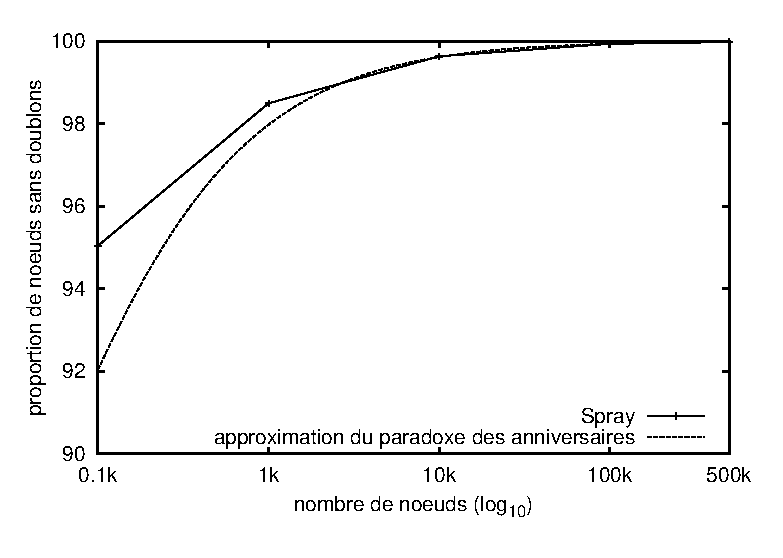
\includegraphics[width=.8\textwidth]{img/spray/duplicates.eps}
  \caption{\label{net:fig:duplicates} Proportion de doublons parmi les nœuds.
    L'axe des abscisses montre la taille du réseau sur une échelle logarithmique
    de base 10. L'axe des ordonnées montre le pourcentage de vues ne possédant
    pas de doublons.}
\end{figure}

Les arcs doublons sont une spécificité de \SPRAY. Ceux-ci permettent de ne pas
perdre d'informations aux cours des mélanges et d'ainsi conserver un nombre
d'arcs cohérent tout au long du cycle de vie du réseau. Toutefois, ils ont un
impact négatif sur certains aspects du réseau : un arc doublon est un arc
n'apportant aucun chemin supplémentaire au réseau. À cet égard, il est important
que le taux de doublons reste faible.

Le paradoxe des anniversaires dit que le nombre de personnes qu'il faut réunir
pour que deux d'entre elles aient le même jour d'anniversaire est, contre toute
attente, faible. À partir de 23 personnes, la probabilité est au dessus de 50\%
et grimpe rapidement. Au delà des anniversaires, ce modèle permet de quantifier
les collisions qu'il peut y avoir lorsque l'on tire des éléments dans un
ensemble borné. Dans notre cas, il est possible d'approximer la probabilité
qu'une vue n'ait pas de doublons par :
\begin{equation*}
  1-
  (1-
  \exp({-\ln(|\mathcal{N}|)*(\ln(|\mathcal{N}|)-1)\over{2*|\mathcal{N}|}}))
\end{equation*}

\begin{itemize}
\item[\textbf{Objectif :}] Montrer que la proportion de doublons dans \SPRAY
  devient négligeable lorsque le réseau grandit.
\item[\textbf{Description :}] Les mesures concernent le nombre de vues
  partielles contenant au moins un doublon après convergence. Celles-ci sont
  effectuées sur des réseaux comprenant 0.1k, 1k, 10k, 100k, et 500k nœuds.
\item[\textbf{Résultat :}] La figure~\ref{net:fig:duplicates} montre la
  proportion de nœuds ne possédant pas de doublons dans leur vue partielle. Nous
  observons qu'il existe toujours au moins une vue partielle contenant un
  doublon. La proportion est plus importante lorsqu'il s'agit de réseaux de
  petite taille (e.g. 5\% pour 100 nœuds). Cette proportion diminue à mesure que
  la taille du réseau grandit (e.g. moins de 1\% à partir de 10k nœuds). La
  figure~\ref{net:fig:duplicates} montre que l'approximation du paradoxe des
  anniversaires est proche des résultats obtenus par simulation confirmant
  empiriquement qu'il existe une relation entre les deux problèmes.
\item[\textbf{Explication :}] Lorsque le réseau grandit, les chances qu'un nœud
  particulier possède plusieurs références à un autre nœud particulier
  deviennent très faibles. En effet, alors que le réseau grandit linéairement,
  l'ensemble des références détenu par un nœud grandit
  logarithmiquement. Contrairement au problème des anniversaires, la diminution
  en proportion n'est pas contre-intuitive au vu des complexités impliquées.
\end{itemize}

%%% Local Variables:
%%% mode: latex
%%% TeX-master: "../../paper"
%%% End:
